% MIT License

% Copyright (c) 2022 Chiyuru

% Permission is hereby granted, free of charge, to any person obtaining a copy of this software and associated documentation files (the "Software"), 
% to deal in the Software without restriction, including without limitation the rights
% to use, copy, modify, merge, publish, distribute, sublicense, and/or sell
% copies of the Software, and to permit persons to whom the Software is
% furnished to do so, subject to the following conditions:

% The above copyright notice and this permission notice shall be included in all copies or substantial portions of the Software.

% THE SOFTWARE IS PROVIDED "AS IS", WITHOUT WARRANTY OF ANY KIND, EXPRESS OR IMPLIED, INCLUDING BUT NOT LIMITED TO THE WARRANTIES OF MERCHANTABILITY,
% FITNESS FOR A PARTICULAR PURPOSE AND NONINFRINGEMENT. IN NO EVENT SHALL THE AUTHORS OR COPYRIGHT HOLDERS BE LIABLE FOR ANY CLAIM, DAMAGES OR OTHER
% LIABILITY, WHETHER IN AN ACTION OF CONTRACT, TORT OR OTHERWISE, ARISING FROM,
% OUT OF OR IN CONNECTION WITH THE SOFTWARE OR THE USE OR OTHER DEALINGS IN THE SOFTWARE.

\documentclass[UTF8]{ctexart}

\usepackage{amssymb}
\usepackage{amsmath}
\usepackage{cases}
\usepackage{cite}
\usepackage{graphicx}
\usepackage[margin=1in]{geometry}
\geometry{a4paper}
\usepackage{fancyhdr}
\pagestyle{fancy}
\fancyhf{}


\title{学习算法报告}
\author{
    刘锦坤
    \\2022013352}
\date{\today}
\pagenumbering{arabic}

\begin{document}

\fancyhead[C]{学习算法报告}
\fancyfoot[C]{\thepage}

\maketitle
\tableofcontents

\section{问题1}

\begin{figure}[h]
    \centering
    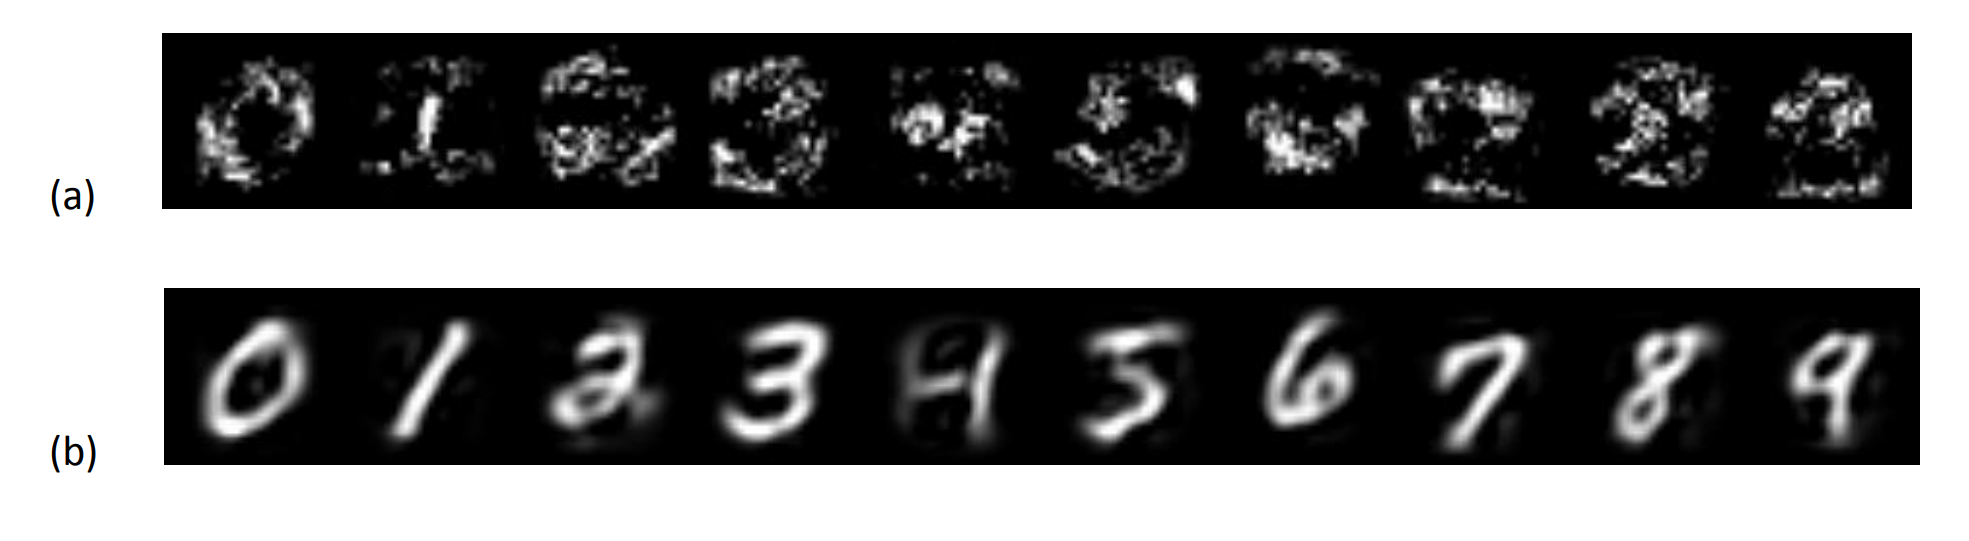
\includegraphics[width=0.8\textwidth]{./image/ab.png}
    \caption{Question1}
    \label{fig:Question1}
\end{figure}

\begin{figure}[h]
    \centering
    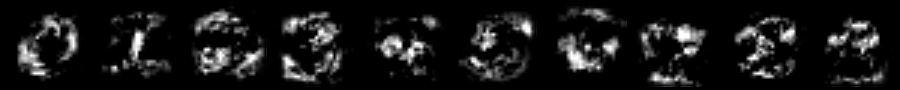
\includegraphics[width=0.8\textwidth]{./image/weights.png}
    \caption{weights.png}
    \label{fig:weights}
\end{figure}

\indent 根据生成的weights.png(如图\ref{fig:weights})可知,Question1中,图\ref{fig:Question1}中的图片(a)更能够代表感知机所学习到的权重矩阵。

\indent 可以看到,各个数字分类的权重向量在可视化后都呈现出对应的数字的轮廓的形状。这是因为对于每个输入数字,要能够将其通过Softmax Regression的方法将其正确分类,就需要其在输出层对应数字位置的值最大。在训练过程中,感知机根据输入的数字的特征,调整权重矩阵,使得输入数字的特征与其对应的权重矩阵的乘积最大,从而使得输出层对应数字位置的值最大。在这个问题中,每个输入的特征就是其各个像素点的值,因此在对应数字越可能出现的位置,权重中对应的值就越大,从而呈现出对应数字的轮廓的形状。

\indent 但是因为即使是对应同一个数字的各个输入中,手写的数字的形状也是有所不同的,因此权重矩阵在可视化后不会表现成一个完全锐利的数字轮廓,而是一个较为模糊的数字轮廓,其反映的事实上是对应数字的各个输入中总体出现的较多的像素点的那些位置,这也就导致对于某些输入,当他们的写法偏离训练的输入写法较大时,不经过或较少经过这些权重矩阵集中分布的像素点,这种情况下,感知机就可能会产生错误的分类判断。

\section{算法分析}

\subsection{K-Means算法}

\indent K-Means算法是一种基于距离的无监督学习算法,其目的是将数据集中的数据点划分为K个簇,使得每个数据点都属于离其最近的簇。

\indent 在Question1中,我们实现了K-Means算法,算法主要分为以下几个步骤:

\begin{enumerate}
    \item 初始化K个簇的中心点,可以随机选择数据集中的K个点作为初始中心点。
    \item 对于数据集中的每个点,计算其与K个簇中心点的距离,将其划分到距离最近的簇中。
    \item 对于每个簇,重新计算其中心点,即将簇中所有点的坐标取平均值作为新的中心点。
    \item 重复2、3步骤,直到达到最大迭代次数。
    \item 输出K个簇的中心点。
\end{enumerate}

\indent 可以看到,最后K-Means算法成功的完成了对数据集的聚类,将数据集中的数据点划分为K个簇,使得每个数据点都属于离其最近的簇,但是也可以看出K-Means算法有以下不足。

\begin{enumerate}
    \item K值的选择:K-Means算法需要事先确定K值,本次是根据数据集的情况选择的K值,实际K值的选择可能要根据聚类相似性关于K值的变化情况来确定(a sharp drop at the optimal number of cluster)。
    \item 对初始中心点的敏感性:K-Means算法对初始中心点的选择是敏感的,本题中指定了随机化种子,但是不同的初始中心点很可能会导致不同的聚类结果。
    \item 对异常值的敏感性:K-Means算法对异常值比较敏感,异常值可能会导致聚类结果的不准确,可能需要数据预处理获得更好的聚类效果。
\end{enumerate}

\subsection{KNN算法}

\indent KNN算法是一种基于距离的有监督学习算法,其目的是对于一个新的数据点,找到与其最近的K个数据点,根据这K个数据点的标签,对新的数据点进行分类。

\indent 在Question2中,我们实现了KNN算法,算法主要分为以下几个步骤:

\begin{enumerate}
    \item 计算新的数据点与数据集中所有数据点的距离。
    \item 找到与新的数据点距离最近的K个数据点。
    \item 根据这K个数据点的标签,对新的数据点进行分类。
    \item 输出新的数据点的分类结果。
\end{enumerate}

\indent 可以看到,最后KNN算法成功的完成了对新的数据点的分类,并且达到了91\%准确率,但是也可以看出KNN算法有以下不足。

\begin{enumerate}
    \item 计算量大:KNN算法需要计算新的数据点与数据集中所有数据点的距离,计算量较大,当数据集较大时,计算时间会较长。
    \item 对K值的选择敏感:KNN算法中对超参数K值的选择是敏感的,K值的选择可能会影响分类结果,需要根据数据集的情况选择合适的K值。
    \item 依赖特征选择:由于KNN算法是基于特征空间中的距离进行分类的,因此对特征选择是敏感的,需要选择合适的特征来进行分类。
\end{enumerate}

\subsection{Softmax Regression算法}

\indent Softmax Regression算法是一种多分类的有监督学习算法,其目的是对于一个新的数据点,找到其在输出层对应数字位置的值最大的位置,从而对新的数据点进行分类。采用Softmax的方法,将输出层的值转化为概率,使得输出层的值和为1且能够进行反向传播计算梯度从而利用梯度下降法计算。

\indent 在Question3中,我们实现了Softmax Regression算法,并且在算法中加入了L2正则化项,以防止过拟合。最终达到87\%的准确率。关于Softmax Regression算法,有如下总结:

\begin{enumerate}
    \item Softmax Regression算法超参数,例如学习率、学习轮次、正则化系数、批次大小,这些都会影响性能,需要根据数据集的情况进行调整。
    \item Softmax Regression算法同样依赖于特征选择,不难看出,如果特征空间中各个分类之间是线性可分的,那么Softmax Regression算法的性能会更好。
    \item Softmax Regression算法对于数据集的分布是敏感的,如果数据集的分布不均匀,那么Softmax Regression算法的性能会受到影响,例如数据集中如果数字1出现得更多,最后的分类结果也会更多的向数字1倾向。
\end{enumerate}

\subsection{SVM算法}

\indent SVM算法是一种有监督学习算法,其目的是找到一个最优的超平面,使得数据点能够被最大间隔分开。SVM算法的优化目标是最大化间隔,同时使得数据点能够被正确分类。

\indent 在Question4中,我们通过调用sklearn库中的SVM算法,实现了对数据集的分类,最终的准确率为93\%,关于SVM算法,有如下总结:

\begin{enumerate}
    \item SVM算法本质上是一种线性分类器,但是通过核函数的选择,可以将SVM算法扩展到非线性分类器,例如多项式核函数、高斯核函数等,这一问中采用的是高斯核函数。
    \item SVM算法对于超参数的选择是敏感的,例如核函数的选择、正则化系数的选择、损失函数的选择,这些都会影响SVM算法的性能,都需要根据数据集的情况进行调整。
    \item SVM算法可以认为是一种最优的Perceptron算法,通过最大化间隔,使得数据点能够被最大间隔分开,从而使得分类效果更好。
\end{enumerate}

\subsection{Better Classifier}

\indent 在这一问中,我们通过pytorch库,搭建了一个深度神经网络,实现了更好的数据集分类,最终的准确率约为98\%,网络结构设置如图\ref{fig:network}所示:

\begin{enumerate}
    \item 经过两层卷积层,每层卷积核的大小为3,步长为1,padding为1,激活函数为ReLU。每层卷积层后接一个最大池化层,池化核的大小为2,步长为2,并在第二层卷积层后添加了dropout防止过拟合。
    \item 然后将卷积层的输出展平,经过三层全连接层,前两层激活函数为ReLU,经过第一层后添加dropout,最后一层全连接层的激活函数为Softmax分类器。
\end{enumerate}

\indent 在训练过程中,如果检测到设备的GPU,就会使用GPU进行训练,否则使用CPU进行训练。在训练过程中,采用了交叉熵损失函数,采用了SGD优化器,超参数设置如下:

\begin{enumerate}
    \item 学习率:0.1
    \item 动量:0.5
    \item 批次大小:200
    \item 学习轮次:200
\end{enumerate}

\indent 可以看到,最终的准确率达到了98\%,相比于之前的分类器,深度神经网络的分类效果更好,这是因为深度神经网络能够学习到更多的特征,从而使得分类效果更好。
% Insert a pdf file
\begin{figure}[h]
    \centering
    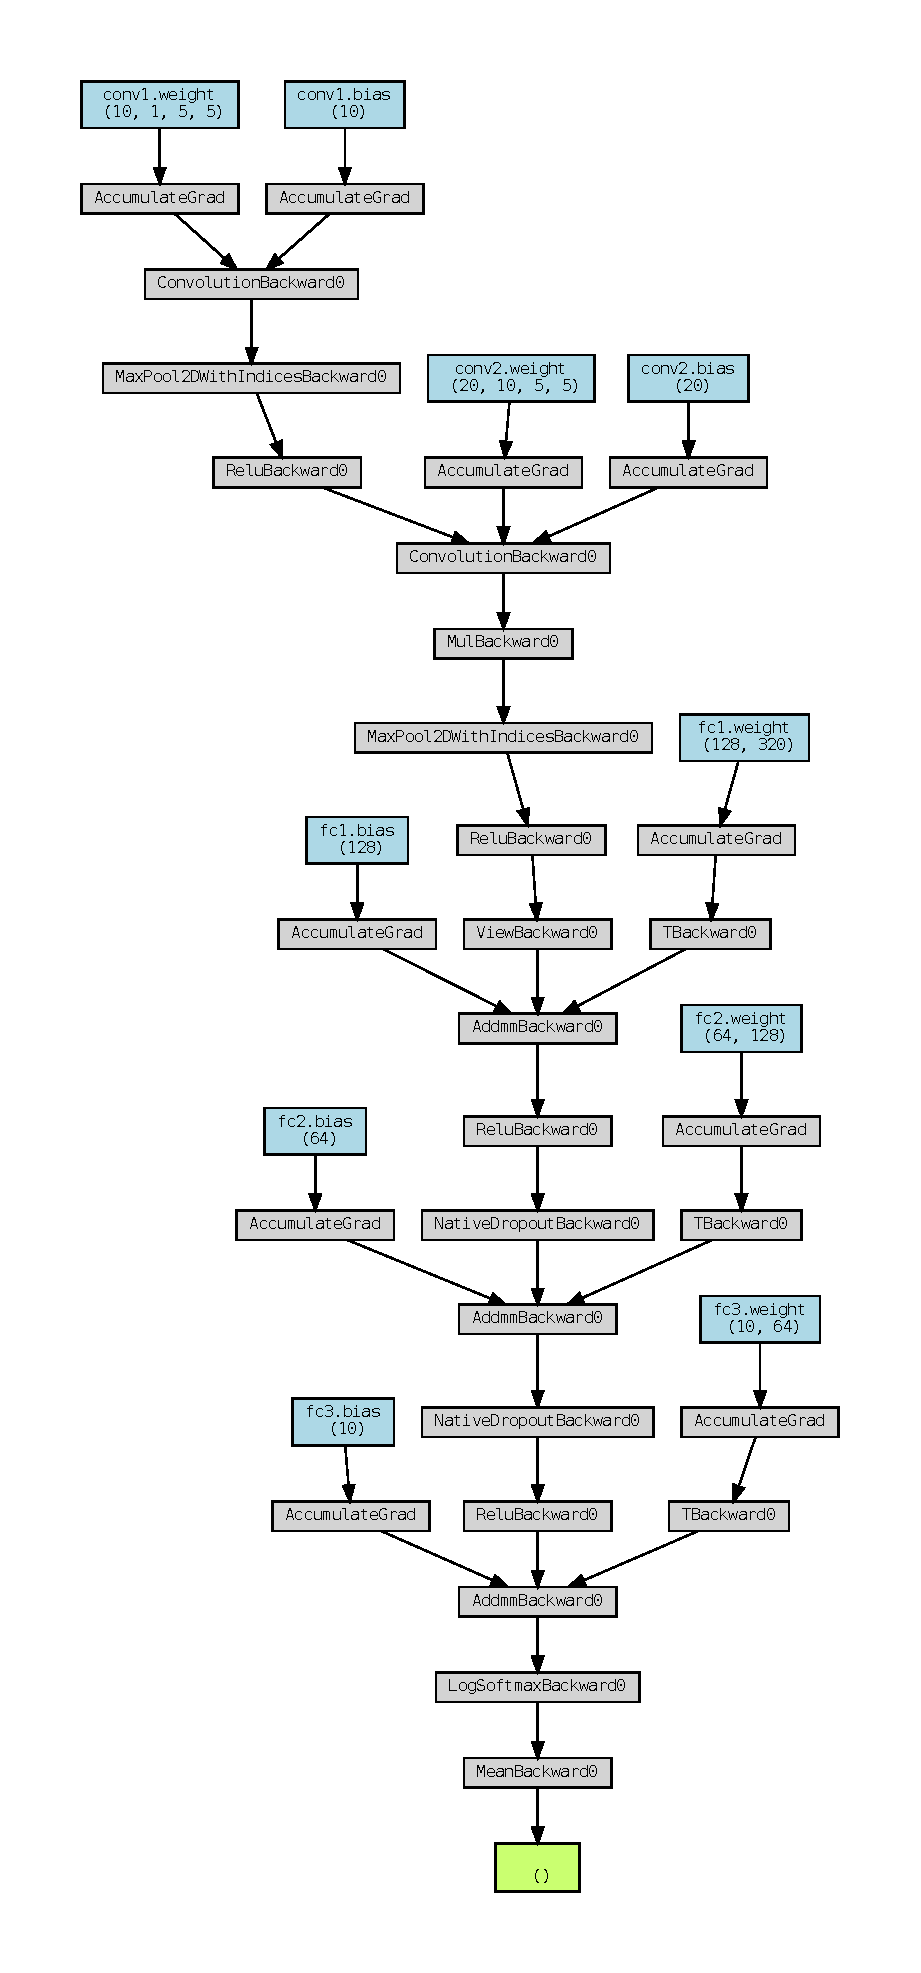
\includegraphics[width=0.7\textwidth]{./image/model.pdf}
    \caption{模型示意图}
    \label{fig:network}
\end{figure}
\end{document} 